\documentclass[12pt]{article}
\usepackage[utf8]{inputenc}
\usepackage[french]{babel}
\usepackage{amsmath,amsthm,amsfonts,amssymb}
\usepackage{lmodern}
\usepackage[top=2.4cm,bottom=2.4cm,left=2cm,right=2cm]{geometry}
\usepackage{hyperref}
\usepackage{multicol}
\usepackage{enumitem}
\usepackage{listings}
\usepackage[dvipsnames]{xcolor}
\usepackage{tikz}
\usepackage{soul}
\date{}
\author{MABROUK Fayez}
\title{{\bf  Génie logiciel} \\
	Rendu de Td \no 11  \\
	{\small L3 Informatique appliquée 2022-2023} \\
	{\it \small \no étudiant : 22213839}}
\begin{document}
	\maketitle
	\newpage
	\section{Projet fil rouge, diagramme de classe}
	
	Partie à faire en trinôme.\\
	\\
	A partir de vos travaux lors des semaines précédentes (définition des exigences, cas d’utilisation et
	diagrammes de séquence), proposez un diagramme de classe pour votre projet. Il est conseillé de
	commencer par lister les classes nécessaires, puis leurs relations et enfin de mettre les attributs et
	méthodes.\\
	\\
	Pour chacune des classes de votre diagramme, vous justifierez sa présence en indiquant comment
	elle a été « découverte ».\\
	\\
	\textbf{Groupe : MABROUK Fayez , AMED-ZAID Macyl , PHAN Dao}
		\begin{figure}[!hbtp]
		\centering
		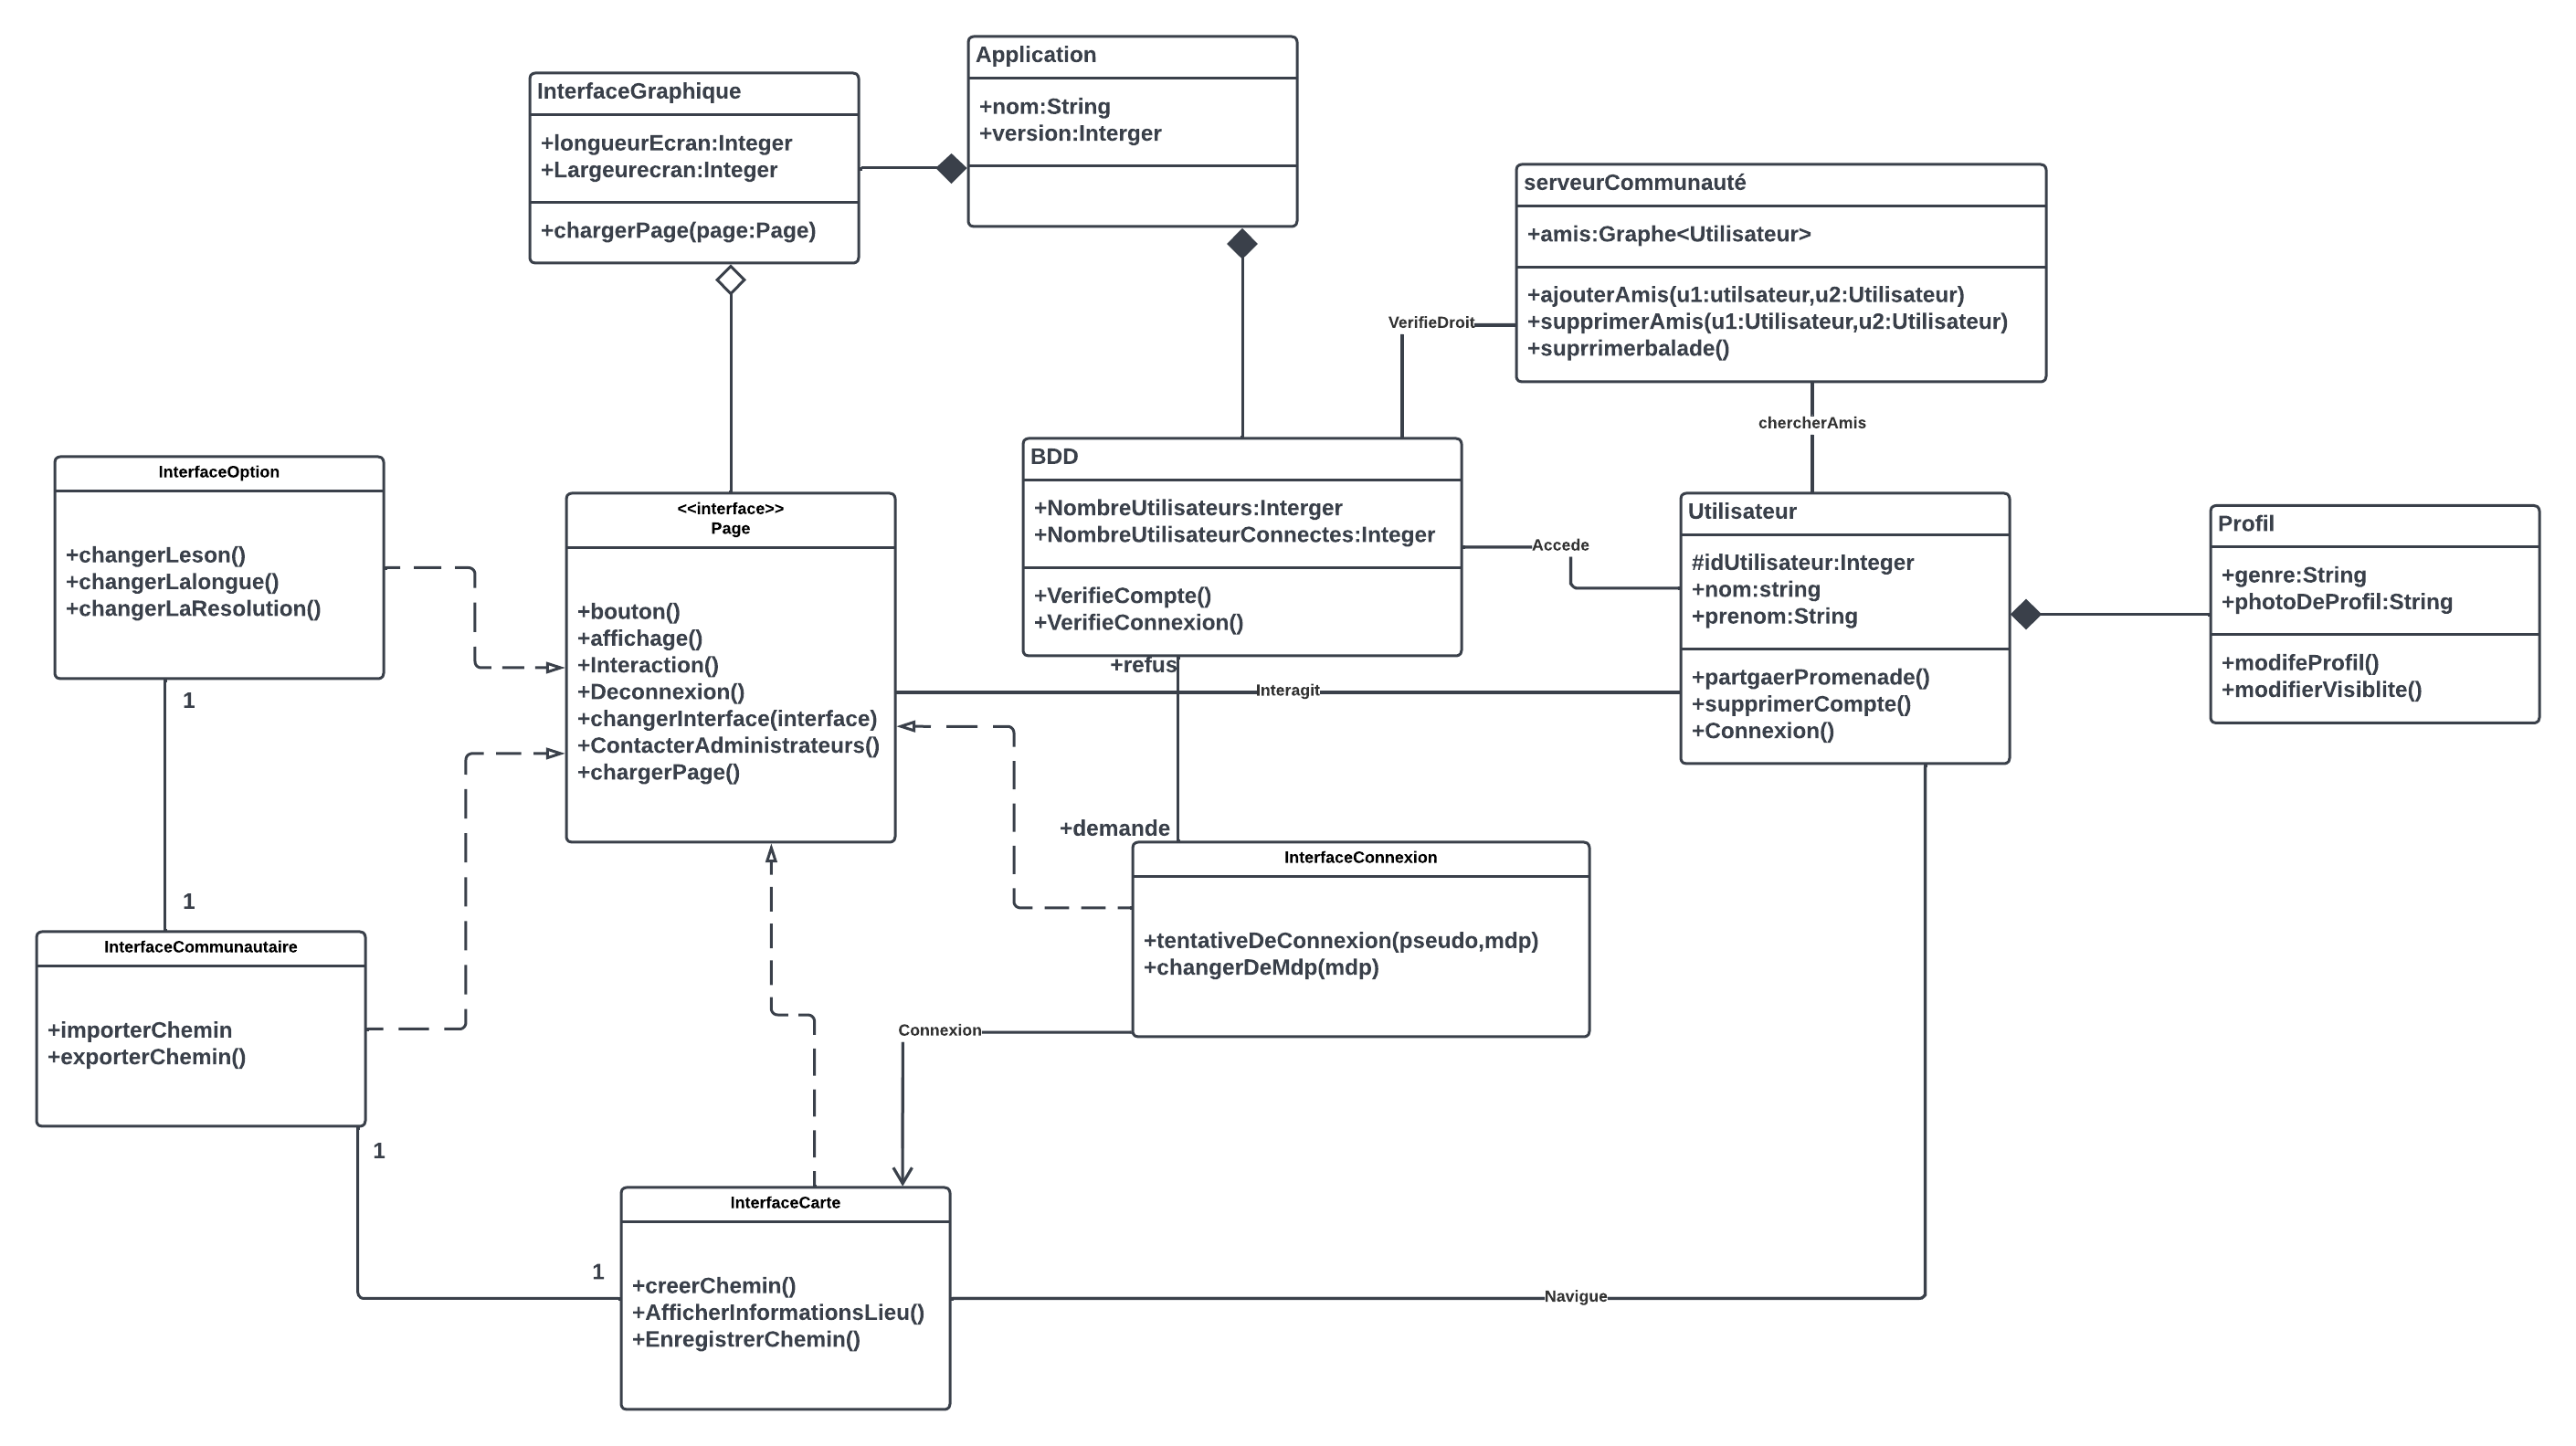
\includegraphics[scale=0.44]{Blank diagram (1).png}
		%\caption{Légende de l'image}
	\end{figure}

\paragraph{\ul{Explications:}}
\begin{itemize}
	\item[* ] Classes \textbf{Application \& Utilisateur} : Application et Utilisateur sont les classes de base de 
	notre modélisation. Elles ont été trouvées à travers les données de l’énoncé du projet.
	\item[* ] Classes \textbf{BDD \& InterfaceGraphique \& InterfaceOption \& \\ InterfaceCommunautaire \& Interface Carte , InterfaceConnexion} : Ces Classes ont été découvertes à partir des 
	diagrammes de séquence.Elles ont été trouvées de façon dynamique. Nous avons commencé 
	par l’acteur principal qui était l’utilisateur, ensuite nous avons analysé avec quoi interagit ce 
	dernier pour trouver les classes une à une.
	\item[* ] Classe \textbf{Page}:Cette Interface modélise l’affichage d’une page au sein de l’application. Une 
	interfaceGraphique contient plusieurs pages. Elle est implémentée par les différentes pages offertes par 
	l’application : InterfaceConnexion, InterfaceCommunautaire, InterfaceCarte
	\item[* ] Classe \textbf{serveurCommunauté}: : Cette classe encapsule toutes les parties en rapport avec les 
	interactions entre des utilisateurs. \\
	\\
	$\Rightarrow$ Nous avons séparé l’utilisateur de son profil pour bien distinguer entre les 
	informations qui caractérisent l’utilisateur au sein de la base de données (minimales) des 
	informations utilisées dans l’aspect communautaire de l’application (comme ses centres 
	d’intérêt) qui pourraient changer régulièrement et qu’il peut choisir de ne pas rendre publics
	
	
	
\end{itemize}
	
\end{document}